\documentclass[a4paper,fleqn,usenatbib]{mnras}

% MNRAS is set in Times font. If you don't have this installed (most LaTeX
% installations will be fine) or prefer the old Computer Modern fonts, comment
% out the following line
\usepackage{newtxtext,newtxmath}
% Depending on your LaTeX fonts installation, you might get better results with one of these:
%\usepackage{mathptmx}
%\usepackage{txfonts}

% Use vector fonts, so it zooms properly in on-screen viewing software
% Don't change these lines unless you know what you are doing
\usepackage[T1]{fontenc}
\usepackage{ae,aecompl}


%%%%% AUTHORS - PLACE YOUR OWN PACKAGES HERE %%%%%

% Only include extra packages if you really need them. Common packages are:
\usepackage{graphicx}	% Including figure files
\usepackage{amsmath}	% Advanced maths commands
\usepackage{amssymb}	% Extra maths symbols
\usepackage{hyperref}
\usepackage{multirow}



\title[Variability in J1100-0053]{A new physical interpretation of optical and infrared variability in quasars}

\author[N.P. Ross et al.]
{Nicholas~P.~Ross$^{1}$\thanks{E-mail: npross@roe.ac.uk},    
K. E. Saavik Ford$^{2,3,4}$,  Matthew Graham$^{5}$,  Barry McKernan$^{2,3,4}$,  
\newauthor Daniel Stern$^{6}$, Aaron M. Meisner$^{7,8}$, Roberto J. Assef$^{9}$, 
Arjun Dey$^{10}$, Andrew J. Drake$^{11}$, 
\newauthor Hyunsung D. Jun$^{12}$, Dustin Lang$^{13,14,15}$
\\
% List of institutions
$^{1}$Institute for Astronomy, University of Edinburgh, Royal Observatory, Blackford Hill, Edinburgh EH9 3HJ, United Kingdom \\
$^{2}$Department of Science, BMCC, City University of New York, New York, NY 10007, USA \\
$^{3}$Department of Astrophysics, Rose Center for Earth and Space, American Museum of Natural History, Central Park West at 79th Street, NY 10024, USA \\
$^{4}$Graduate Center, City University of New York, 365 5th Avenue, New York, NY 10016, USA\\
$^{5}$Cahill Center for Astronomy and Astrophysics, California Institute of Technology, Mail Code 249/17, 1200 E California Blvd, Pasadena CA 91125, USA\\
$^{6}$Jet Propulsion Laboratory, California Institute of Technology, 4800 Oak Grove Drive, Mail Stop 169-221, Pasadena, CA 91109, USA \\
$^{7}$Lawrence Berkeley National Laboratory, 1 Cyclotron Road, Berkeley, CA 92420, U.S.A. \\
$^{8}$Berkeley Center for Cosmological Physics, Berkeley, CA 94720, USA\\
$^{9}$N\'ucleo de Astronom\'ia de la Facultad de Ingenier\'ia y Ciencias, Universidad Diego Portales, Av. Ej\'ercito Libertador 441, Santiago, Chile.\\
$^{10}$National Optical Astronomy Observatory, 950 N. Cherry Ave, Tucson, AZ 85719, USA \\
$^{11}$Center for Advanced Computing Research, California Institute of Technology, 1200 E California Blvd, Pasadena CA 91125, USA \\
$^{12}$School of Physics, Korea Institute for Advanced Study, 85 Hoegiro, Dongdaemun-gu, Seoul 02455, Korea\\
$^{13}$Dunlap Institute, University of Toronto, Toronto, ON M5S 3H4, Canada \\
$^{14}$Department of Astronomy \& Astrophysics, University of Toronto, Toronto, ON M5S 3H4, Canada \\
$^{15}$Perimeter Institute for Theoretical Physics, Waterloo, ON N2L 2Y5, Canada\\
}

\date{Accepted XXX. Received YYY; in original form ZZZ}
\pubyear{2018}

%\hypersetup{draft}
\begin{document}
\label{firstpage}
\pagerange{\pageref{firstpage}--\pageref{lastpage}}
\maketitle


\begin{abstract}
Changing-look quasars are a recently identified class of active
galaxies in which the strong UV continuum and/or broad optical
hydrogen emission lines associated with unobscured quasars either
appear or disappear on timescales of months to years.  The physical
processes responsible for this behaviour are still debated, but
changes in the black hole accretion rate or accretion disk structure
appear more likely than changes in obscuration.  Here we report on
four epochs of spectroscopy of SDSS J110057.70-005304.5, a quasar at a
redshift of $z=0.378$ whose UV continuum and broad hydrogen emission
lines have faded, and then returned over the past $\approx$20
years. The change in this quasar was initially identified in the
infrared, and an archival spectrum from 2010 shows an intermediate
phase of the transition during which the flux below rest-frame
$\approx$3400\AA\ has decreased by close to an order of magnitude. This
combination is unique compared to previously published examples of
changing-look quasars, and is best explained by dramatic changes in
the innermost regions of the accretion disk. The optical continuum has
been rising since mid-2016, leading to a prediction of a rise in
hydrogen emission line flux in the next year. {\bf Increases in the
infrared flux are beginning to follow}, occurring on a $\sim$3 year observed
timescale. If our model is confirmed, the physics of changing-look
quasars are governed by processes at the innermost stable circular
orbit (ISCO) around the black hole, and the structure of the innermost
disk. The easily identifiable and monitored changing-look quasars
would then provide a new probe and laboratory of the nuclear central
engine.
\end{abstract}

% Select between one and six entries from the list of approved keywords.
% Don't make up new ones.
\begin{keywords}
accretion, accretion discs -- surveys -- quasars: general
\end{keywords}




%%%%%%%%%%%%%%%%%%%%%%%%%%%%%%%%%%%%%%%%%%%%%%%%%%%%%%%%%%%%%%%%%%%%%%%%%%%%%%%%%
%%%%%%%%%%%%%%%%%%%%%%%%%%%%%%%%%%%%%%%%%%%%%%%%%%%%%%%%%%%%%%%%%%%%%%%%%%%%%%%%%
%%
%%
%%   SECTION 1  SECTION 1  SECTION 1  SECTION 1  SECTION 1  SECTION 1  
%%   SECTION 1  SECTION 1  SECTION 1  SECTION 1  SECTION 1  SECTION 1  
%%   SECTION 1  SECTION 1  SECTION 1  SECTION 1  SECTION 1  SECTION 1  
%%
%%
%%%%%%%%%%%%%%%%%%%%%%%%%%%%%%%%%%%%%%%%%%%%%%%%%%%%%%%%%%%%%%%%%%%%%%%%%%%%%%%%%%
%%%%%%%%%%%%%%%%%%%%%%%%%%%%%%%%%%%%%%%%%%%%%%%%%%%%%%%%%%%%%%%%%%%%%%%%%%%%%%%%%%
\section{Introduction}
{\bf 
The Shakura-Sunyaev $\alpha-$disk model \citep{SS73} has long been used to describe the basic properties of the optically thick, geometrically thin accretion disks expected to orbit the supermassive black holes at the nuclei of quasars. This accretion disk is thought to be the origin of thermal continuum emission observed in the rest-frame ultraviolet and optical. The thermal emission seen in the infrared spectrum of quasars is believed to originate from molecular dust outside the accretion disk and traditional broadline region (BLR). Thus, the IR flux is directly proportional to the emission from the disk, reprocessed by the dusty reservoir and delayed by the light-travel time between the two \citep[see e.g.,][for reviews]{Antonucci1993, Perlman2008, Lasota2016}. As such, the thermal accretion disk photons are the seeds for both the X-ray emission -- due to Compton-upscattering in the corona \citep[e.g.,][]{Begelman1983, Risaliti2009, Lusso2017} and the thermal mid-IR emission from the torus.

The $\alpha$-disk model assumes that the disk is geometrically thin (i.e., $h/r \ll 1$ where $h/r$ is the disk aspect ratio) and that angular momentum is transported by a kinematic viscosity, $\nu$, parametrized by \citet{SS73} as $\nu = \alpha c_{\rm s} h$ where $c_{\rm s}$ is the local mean sound speed in the disk and $h$ is the scale-height perpendicular to the disk plane. The thermal emission need not be, but often is, treated as a superposition of blackbodies at varying annuli with an effective temperature dependence\footnote{This r$^{-3/4}$ temperature dependence is not specific to the $\alpha$-parametrization, and is independent from the nature of the viscosity, provided that the disk is geometrically thin, steady and heat dissipation and angular momentum transport and caused by the same, local mechanism.} going as $T(r) \propto r^{-3/4}$. 
%The $\alpha-$disk model makes the key assumptions that plasma within the disk is optically thick and thermal, and emission from the accretion disk can be treated as a superposition of blackbody annuli. h/r

Given the size scales and temperatures associated with supermassive black holes, a substantial fraction of the bolometric luminosity should be in the form of UV photons --  the so-called ``Big Blue Bump'' \citep{Shields1978, Malkan_Sargent1982}. For the optically thick, UV emitting disk to accrete onto the black hole, substantial angular momentum must be lost.  The kinematic viscosity of the plasma, $\alpha$, seems the likely mechanism that transports angular momentum outward.  This viscosity is likely due to magnetorotational instability \citep[MRI; ][]{Balbus_Hawley1991} with additional contributions to turbulence from the effects of objects embedded in the disk \citep[e.g.,][]{McKernan2014}. 

However, as has long been established \citep[e.g., ][]{Alloin1985} and recently re-visited \citep[e.g., ][]{LaMassa2015, Runnoe2016, MacLeod2016, Ruan2016, Rumbaugh2017, Yang2017, Lawrence2018}, the observation of even slowly varying Balmer emission lines in quasars strongly suggests that if a thermal accretion disk does indeed contribute substantially to the ionizing or optical continuum, then it cannot be in quasi-steady state equilibrium. The variations must be due to more chaotic disturbances or instabilities in the disk that propagate at considerably higher speeds than the radial accretion flow and possibly as fast as the orbital velocity.

Furthermore as e.g., \citet{Koratkar_Blaes1999} and \citet{Sirko_Goodman2003} among others point out, the observed spectral energy distributions (SEDs) of typical quasars differ markedly from classical $\alpha$-disk theoretical predictions \citep[][]{SS73, Pringle1981} with a typical observed quasar SED flat in $\lambda F_{\lambda}$ over several decades in wavelength \citep{Elvis1994, Richards2006b}. Also, real AGN disks seem to be cooler \citep[e.g., ][]{Lawrence2012} and larger \citep[e.g.,][]{Pooley2007, Morgan2010, Morgan2012, Mosquera2011} than the $\alpha$-disk model predicts. The $\alpha$-disk is an ad hoc parameterization of disk viscosity and does not permit predictions of global changes from local perturbations \citep{King2012}. 

Nevertheless, in this paper, we utilize the mathematically simple $\alpha$-disk model as a framework and departure point for our own disk models. Here, we build on previous work \citep{Sirko_Goodman2003, Zimmerman2005, Hameury2009} and introduce a phenomenological model which does allow changes across the accretion disk and, crucially, makes predictions which can be observed in the SED.
}

Changing-look quasars (CLQs) are luminous active galaxies in which the
strong UV continuum and/or broad optical hydrogen emission lines
associated with unobscured quasars either appear or disappear on
timescales of months to years. CLQs have traditionally been discovered
by looking for large, $| \Delta m | >1$ magnitude changes in the
optical light curves of quasars or galaxies. In contrast, we have
taken advantage of the ongoing mid-IR Near-Earth Object Wide-Field
Infrared Survey Explorer Reactivation mission \citep[NEOWISE-R;
][]{Mainzer2014, Meisner2017a, Meisner2017b}, supplemented with the
optical Dark Energy Camera Legacy Survey (DECaLS\footnote{{\tt
legacysurvey.org/decamls/}}), in order to discover new changing-look
quasars.  While previous efforts have used the 1-year baseline of the
WISE mission to identify changing-look quasars
\citep[e.g.,][]{Assef2018, Stern2018}, our investigation is the first
to extend this selection to the infrared using NEOWISE-R mission
data. We have identified a sample of Sloan Digital Sky Survey (SDSS)
quasars that show significant changes in their IR flux over the course
of a few years. Importantly, our IR light curves enable us to set
limits on SED changes due to obscuration.

In this article we present the $z=0.378$ quasar SDSS J110057.70-005304.5 (hereafter J1100-0053).  J1100-0053 was a known quasar we identified as interesting due to its IR light curve. We have spectral observations for J1100-0053 showing a transition in the blue-continuum into a `dim state' where the rest-frame UV flux is suppressed, and then returning to a blue-continuum sloped quasar.  The model we present invokes changes at {\bf the Innermost stable circular orbit (ISCO, defined as $r_{\textsc{ISCO}}={\frac {6\,GM}{c^{2}}}$ in the Schwarzschild metric),} to be the triggering event for substantial changes in the wider accretion disk, including major structural changes out to 150$r_{g}$ (where $r_{\rm g}$ is the gravitational radius; $r_{\rm g}=\frac{GM}{c^2}$). Such a model explains changes in the broad emission lines, as well as the optical and IR light curves.

{\bf This paper is organised as follows.  In Section 2, we describe
our sample selection, catalogs and observationa data sets.  In Section
3, we present various theoretical models and discuss if and how each
describes and explains the data.  We conclude in Section 4.}  We
report all magnitudes on the AB zero-point system \citep{Oke_Gunn1983,
Fukugita1996}.  For the WISE bands, $m_{\rm AB} = m_{\rm Vega} + m$
where $m = (2.699, 3.339)$ for WISE W1 at 3.4$\mu$m and WISE W2 at
4.6$\mu$m, respectively \citep{Cutri2011}. {\bf We choose the
cosmological parameters $\Omega_{\Lambda} = 0.7$, $\Omega_{\rm M} =
0.3$, and $h = 0.7$ in order to be consistent with \citet{Shen2011}}.


\begin{figure*}
  \centering
  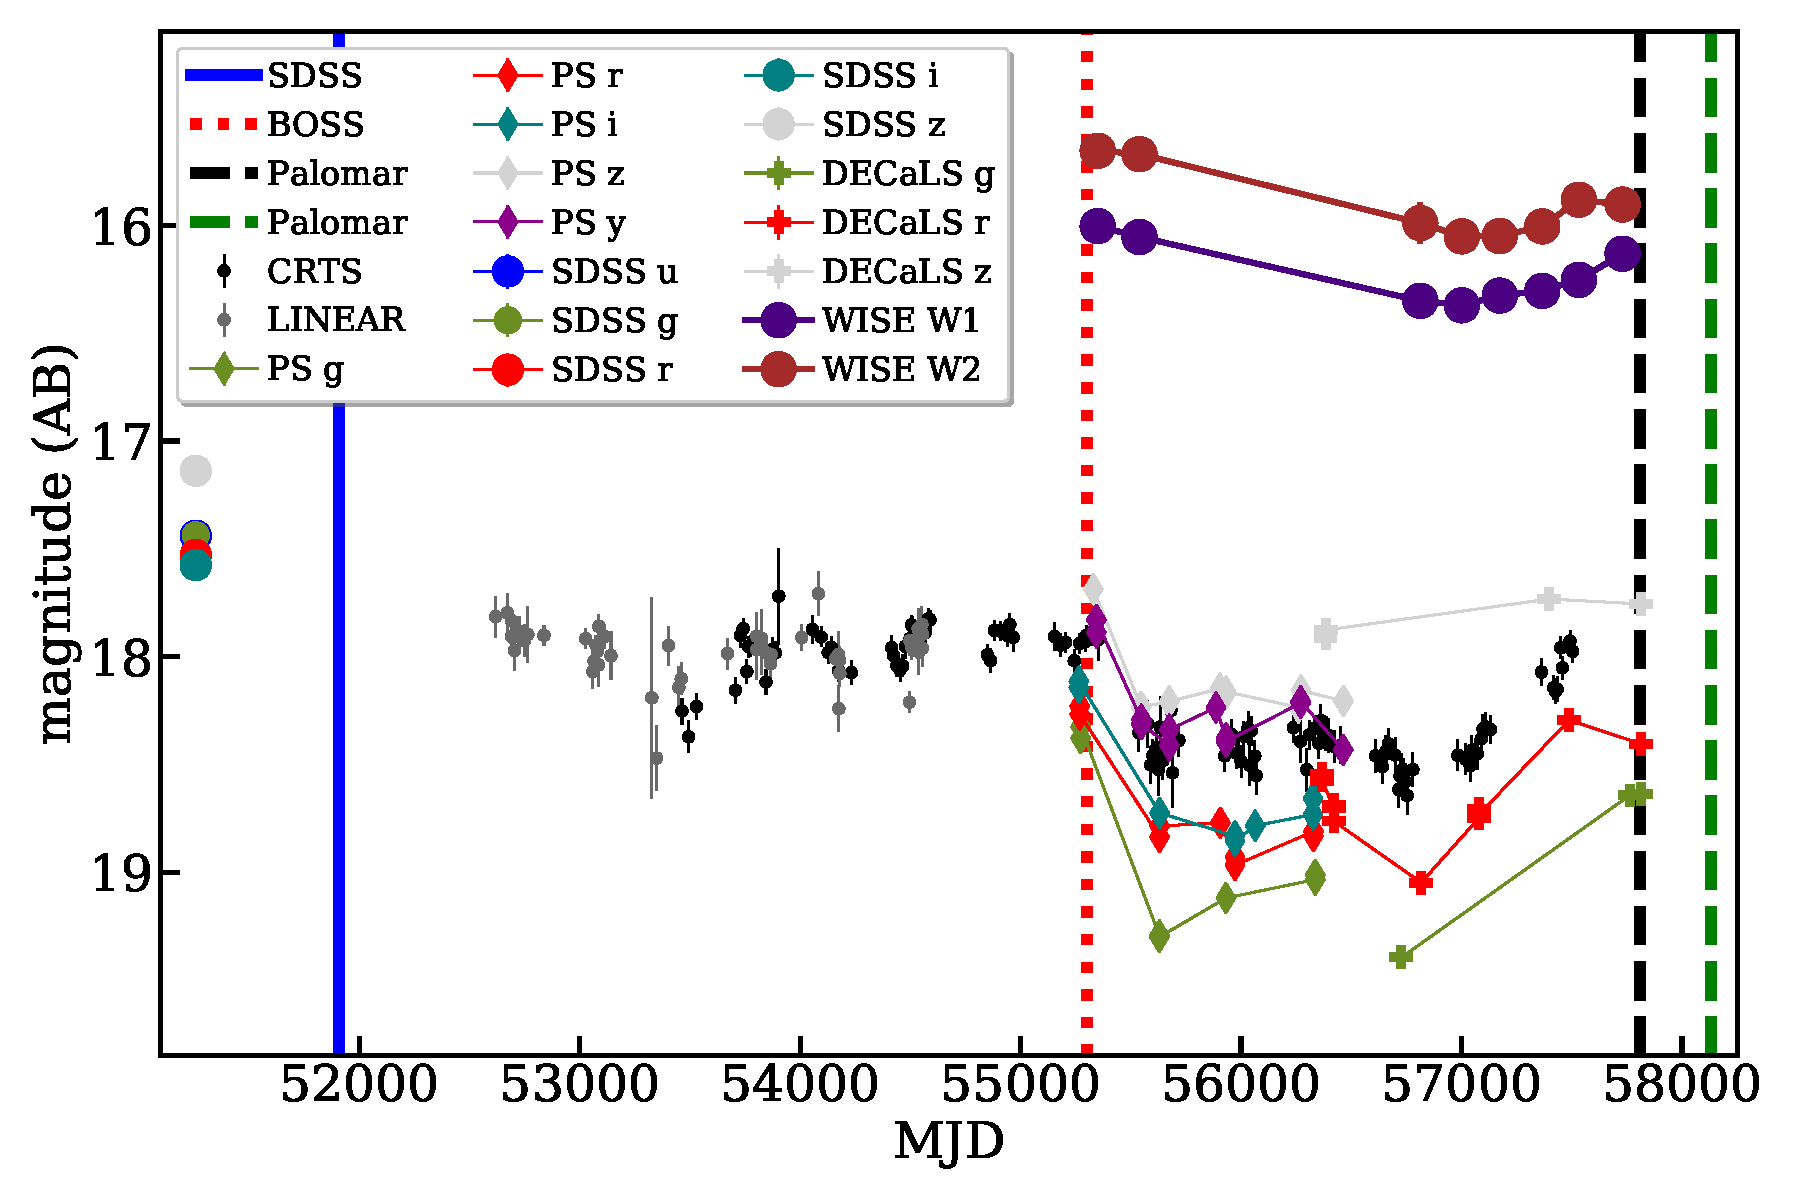
\includegraphics[width=16.00cm, height=11.00cm, trim=0.0cm 0.0cm 0.0cm 0.0cm, clip]
  {../plots/lc/J110057_lc_20180501.pdf}
  \caption[]{
    Multi-wavelength light curve of J1100-0053, including optical data
    from LINEAR, CRTS, SDSS, PanSTARRS and DECaLS, and mid-IR data from
    the WISE satellite.  The four vertical lines illustrate the four
    epochs of optical spectra presented in Figure 2.  J1100-0053 was
    flagged for further study due to the IR fading observed by WISE.  Note
    that the optical emission has been recovering over the past few years,
    with the IR emission beginning to show similar behvaiour. The inserts
    show the images of J1100-0053 from SDSS in 1999 March and the DECaLS DR3
    in 2014 March (50'' on a side). }
  \label{fig:J110057_LC_CRTS}
\end{figure*}
%%%%%%%%%%%%%%%%%%%%%%%%%%%%%%%%%%%%%%%%%%%%%%%%%%%%%%%%%%%%% 
%%%%%%%%%%%%%%%%%%%%%%%%%%%%%%%%%%%%%%%%%%%%%%%%%%%%%%%%%%%%% 
%%
%%
%%     SECTION 2   SECTION 2   SECTION 2   SECTION 2   SECTION 2   SECTION 2  
%%     SECTION 2   SECTION 2   SECTION 2   SECTION 2   SECTION 2   SECTION 2  
%%     SECTION 2   SECTION 2   SECTION 2   SECTION 2   SECTION 2   SECTION 2  
%%
%%
%%%%%%%%%%%%%%%%%%%%%%%%%%%%%%%%%%%%%%%%%%%%%%%%%%%%%%%%%%%%%
%%%%%%%%%%%%%%%%%%%%%%%%%%%%%%%%%%%%%%%%%%%%%%%%%%%%%%%%%%%%%
\section{Target Selection and Observations}  

\subsection{Selection in SDSS and NEOWISE-R of J1100-0053}
We started by matching the SDSS Data Release 7 \cite[DR7Q;
][]{Schneider2007} and the SDSS-III Baryon Oscillation Spectroscopic
Survey (BOSS) Data Release 12 Quasar catalogues \cite[DR12Q;
][]{Paris2017} to the NEOWISE-R IR data. We use data from the
beginning of the WISE mission \citep[2010 January; ][]{Wright2010}
through the thrid-year of NEOWISE-R operations \citep[2016 December;
][]{Mainzer2011}. The WISE scan pattern leads to coverage of the
full-sky approximately once every six months (a ``sky pass''), but the
satellite was placed in hibernation in 2011 February and then
reactivated in 2013 October. Hence, our light curves have a cadence of
6 months with a 32 month sampling gap.

The W1/W2 light curves for $\sim$200,000 SDSS and BOSS spectroscopic
quasars were obtained by performing forced photometry at the locations
of DECam-detected optical sources \citep{Lang2014, Meisner2017a,
Meisner2017b}. This forced photometry was performed on time-resolved
coadds \citep{Lang2014}, each of which represents a stack of $\sim$12
exposures. The coaddition removes the possibility of probing
variability on $\lesssim$1 day time scales, but pushes $\approx$1.4
magnitudes deeper than individual exposures while removing virtually
all single-exposure artifacts (e.g. cosmic rays and satellites).

Approximately $\sim$30,000 of the SDSS/BOSS quasars with W1/W2
light-curves available are `IR-bright', in that they are above both
the W1 and W2 single exposure thresholds and therefore detected at
very high significance in the coadds. For this ensemble of objects,
the typical variation in each quasar's measured (W1-W2) color is 0.06
magnitudes.  This includes statistical and systematic errors which are
expected to contribute variations at the few hundredths of a magnitude
level. The typical measured single-band scatter is 0.07 magnitudes in
each of W1 and W2.

We undertook a search for outliers relative to these
trends. Specifically, we selected objects with the following
characteristics:
\begin{itemize}
  \item Monotonic variation in both W1 and W2 flux.
  \item W1 flux and W2 flux Pearson correlation coefficient $r \geq0.9$.
  \item $>$0.5 mag peak-to-peak variation in either W1 or W2.
\end{itemize}
This yields a sample of 248 sources. 31 of these are assumed to be
blazars due to the presence of Faint Images of the Radio Sky at
Twenty-Centimeters \citep[FIRST; ][]{Becker1995} radio counterparts,
and we discount them for further analyses. Another 22 objects are
outside the FIRST footprint, leaving 195 quasars in our IR-variable
sample, with no potential FIRST counterparts detected within 30''. 

Although aperture photometry and DECaLS forced photometry
\citep{Lang2014, Meisner2017a, Meisner2017b} are available, J1100-0053
is significantly above the single-exposure detection limit so it is
valid to obtain photometry from the publicly released W1/W2 Level 1b
(L1b) single-exposure images at the NASA/IPAC Infrared Science Archive
(\href{http://irsa.ipac.caltech.edu/}{IRSA}).  Upon querying the
combined the WISE All-Sky, WISE Post-Cryo and NEOWISE-R databases, we
have 101 measurements in 8 sky passes spanning nearly 2400 days.

Links to all our data, catalogs and analysis can be found
online at: \href{https://github.com/d80b2t}{{\tt github.com/d80b2t}}.


\subsection{Optical Imaging}
Figure~\ref{fig:J110057_LC_CRTS} presents the light curve of SDSS
J110057.70-005304.5.  J1100-0053 was first detected in the National
Geographic Society-Palomar Observatory Sky Survey \cite[NGS-POSS;
][]{Abell1959, Minkowski_Abell1963book} in 1955 April. It is
catalogued in the SuperCOSMOS Science Archive
\citep[\href{http://ssa.roe.ac.uk/}{SSA}; ][]{Hambly2001_I,
Hambly2001_II} and due to its equatorial position was also observed by
the UK Schmidt Telescope \cite[UKST; ][]{Cannon1975,
Cannon1979book}. Querying the SSA returns {\it gCorMag} and {\it
sCorMag} which are the magnitudes assuming the object is either a
galaxy or star, respectively. We use the {\it sCorMag} values as is
appropriate for an image with flux dominated by the point-like AGN;
the {\it sCorMag} magnitudes are calibrated in the Vega system. For
J1100-0053 we find the magnitudes are: 18.10 mag in the blue UK-J
filter from MJD 45440.47 (1983 April 16); 17.49 mag in the red POSS-I
'E'-filter from MJD 35214.22 (1955 April 17); 17.92 mag in the red
UK-R filter from MJD 46521.47 (1986 April 01) and 17.71 mag in the
UK-I filter from MJD 47273.49 (1988 April 22). J1100-0053 is not in
the Digital Access to a Sky Century @ Harvard
(DASCH\footnote{http://dasch.rc.fas.harvard.edu/project.php}).

J1100-0053 was imaged by the Sloan Digital Sky Survey (SDSS) in the
$u$, $g$, $r$, $i$ and $z$-bands in 1999 March, and more recently by
the Dark Energy Camera Legacy Survey (DECaLS) where there are 4, 13
and 4 exposures in the $g$, $r$ and $z$-bands, respectively, in the
DECaLS Data Release 3 \citep[DR3; ][]{Dey2018}. The $g$-band
observations span $\approx$3 years ($56727 \leq g_{\rm MJD} \leq
57816$), while the $r$- and $z$-band observations span $\approx$4
years ($56367 \leq r_{\rm MJD} \leq 57814$ and $56383 \leq z_{\rm MJD}
\leq 57815$).

Along with WISE IR data, optical data from the SDSS, Catalina
Real-time Transient Survey \citep[CRTS;][]{Drake2009, Mahabal2011},
the Lincoln Near-Earth Asteroid Research \citep[LINEAR; ][]{Sesar2011}
program and the Panoramic Survey Telescope and Rapid Response System
\citep[PanSTARRS;][]{Kaiser2010, Stubbs2010, Tonry2012, Magnier2013}
are also available, and presented in Fig.~\ref{fig:J110057_LC_CRTS}.




\begin{figure*}
  \centering
  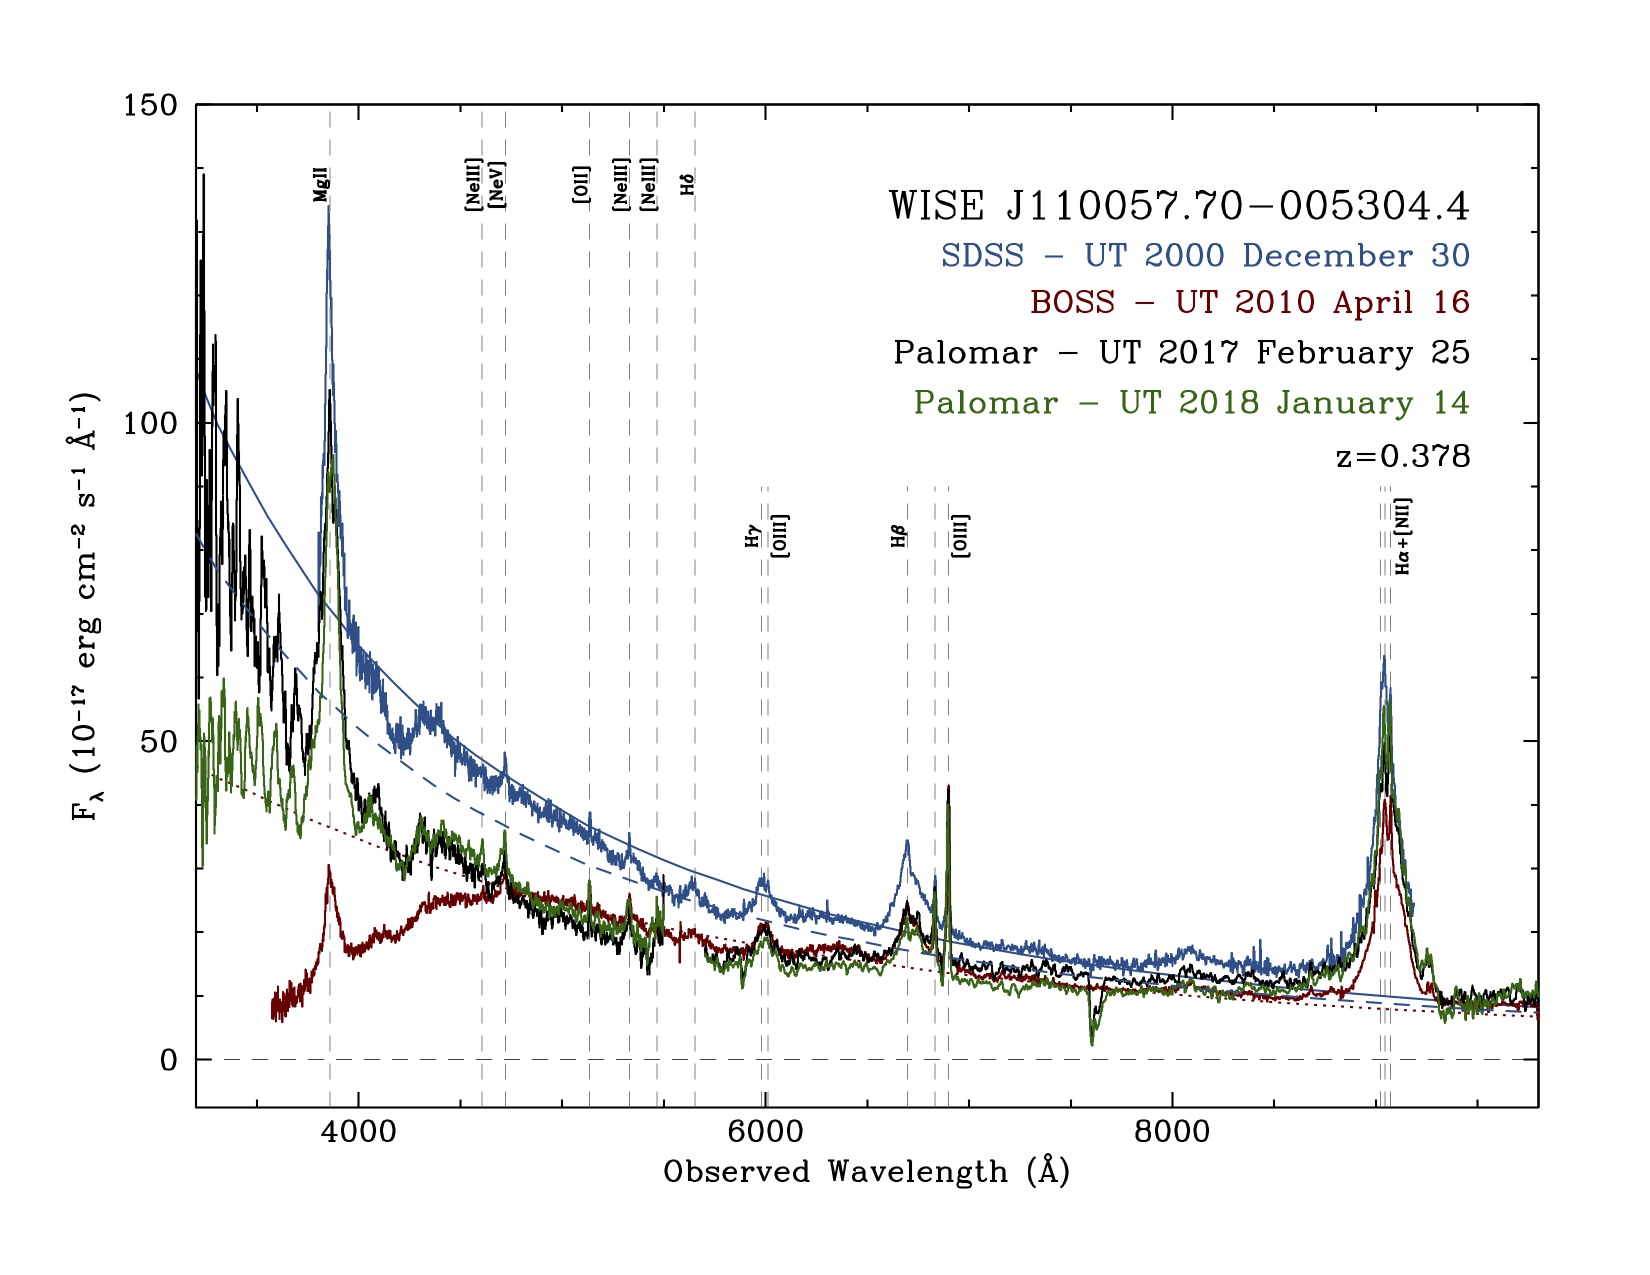
\includegraphics[width=17.00cm, trim=0.0cm 0.0cm 0.0cm 0.0cm, clip]
  {../plots/spectra/w1100m0053_sdss_palomar2.jpg}
\vspace{-16pt}
  \caption[]{
    Optical spectra of J1100-0053 obtained on MJD 51908 (blue; SDSS),
    55302 (red; BOSS), 57809 (black; Palomar) and 58132 (green;
    Palomar). Spectra have been renormalized to maintain a constant
    [O\,{\sc iii}]\ luminosity. Over the past two decades, the UV
    continuum and broad lines have changed significantly for this quasar.
    In particular, the 2nd-epoch BOSS spectrum from 2010 shows the rare
    occurrence of a temporary collapse of the UV continuum.  Smooth lines
    show three simple thermal accretion disk models of the continuum.  The
    solid blue line shows an inflated disk with non-zero torque at the
    ISCO \cite[e.g.,][]{Sirko_Goodman2003}, while the dashed blue line
    shows the same model, but with zero torque at the ISCO \cite[i.e.,
    equivalent to a simple $\alpha$-disk model,][]{SS73}.  Torque at the
    ISCO, possibly due to magnetic fields threading the inner disk and
    plunging region, heats the inner disk, causing it to puff up and
    become more UV luminous.  The dotted red line shows a modified
    zero-torque model where the thermal disk emission interior to $80
    r_{\rm g}$ is suppressed by a factor of 10.}
  \label{fig:J110057_spectra}
\end{figure*}
\subsection{Additional Multiwavelength Data for J1100-0053}
J1100-0053 was observed by R\"{o}ntgensatellit (ROSAT) and appears in
the All-Sky Survey Bright Source Catalogue \citep[RASS-BSC;
][]{Appenzeller1998, Voges1999} as 2RXS J110058.1-005259 with 27.00
counts (count error 6.14) and a count rate = 0.06$\pm$0.01
counts~s$^{-1}$ \citep{Boller2016}. The NASA/IPAC Extragalactic
Database (NED\footnote{https://ned.ipac.caltech.edu/}) gives
J1100-0053 as having a flux $1.27\pm0.28 \times^{-12}$ erg cm$^{-2}$
s$^{-1}$ in the 0.1-2.4 keV range (unabsorbed). J1100-0053 is not in
either the {\it Chandra} or XMM-{\it Newton} archives but is detected
by the Galaxy Evolution Explorer \citep[GALEX; ][]{Martin2005,
Morrissey2007} and has reported flux densities $19.29\pm0.12$ mag in
the far-UV and $18.89\pm0.05$ mag in the near-UV. As noted above,
there is no radio counterpart within 30 arcsec in the FIRST survey,
i.e. at 21cm. None of the {\it Hubble Space Telescope}, {\it Spitzer
Space Telescope} or {\it Kepler} missions have observed J1100-0053.
It is also not in the Hyper Suprime-Cam (HSC)
\href{https://hsc-release.mtk.nao.ac.jp/doc/}{Data Release 1}
\citep{Aihara2017} footprint.


{\bf 
  \begin{table}
    \centering
    \begin{tabular}{l r r r}
      \hline \hline 
       Spectrum                                                        &	SDSS  &	BOSS    &	Palomar\\
      MJD                                                                  &    51908 &  55302  &    57809          \\              
      \hline   
       Equivalent Widths & & & \\   
     H$\gamma$                                                       &    23       &   23    &    30 \\
      H$\beta$ +  [O\,{\sc iii}]                                   &  132       & 124    &  101 \\
        $\lambda$4959 [O\,{\sc iii}]                           &      5       &     7    &   11 \\
         $\lambda$5007 [O\,{\sc iii}]                          &    16      &  25 &     26\\
      H$\beta$                                                           &  111     &   92   &    65\\
     $^{{\rm a}}$H$\alpha$+[NII]:                                 &  390     &  530    &   462\\
      \hline   
      Line Ratios  & & & \\
      H$\beta$      / (H$\alpha$ + [N\,{\sc ii}])   &  0.36    &  0.27   &  0.18 \\
      H$\gamma$ / (H$\alpha$ + [N\,{\sc ii}])   &  0.09    &  0.08   &  0.08 \\
      H$\beta$      / [O\,{\sc iii}]   	                  &  6.03    &  3.08   &  1.80  \\ 
      H$\gamma$ / H$\beta$      	                  &  0.24    &  0.28   &  0.45 \\
      \hline \hline 
  \end{tabular}
      \caption{Approximate Equivalent Width and emission line ratios for J1100-0053.
        Equivalent Widths are in Angstroms. 
        $^{{\rm a}}$Estimated by extrapolating the H$\alpha$ line, which is partially truncated at edge of spectrum.} 
      \label{tab:line_ratios}
\end{table}
}

\subsection{Spectroscopy}
\subsubsection{SDSS and BOSS Spectroscopy}

Figure~\ref{fig:J110057_spectra} shows the four optical spectra of
J1100-0053. J1100-0053 satisfied a number of spectroscopic targeting
flags making it a quasar target in SDSS \citep{Richards2002}. An SDSS
spectrum was obtained on MJD 51908 (SDSS Plate 277, Fiber 212) and the
spectrum of a $z=0.378$ quasar was catalogued in the SDSS Early Data
Release \citep{Stoughton2002, Schneider2002}.

The second epoch spectrum is from the SDSS-III Baryon Oscillation
Spectroscopic Survey \citep[BOSS; ][]{Dawson2013} on MJD 55302 and
shows the downturn at $\lesssim$4300\AA\ (observed). SDSS-III BOSS
actively vetoed previously known $z<2$ quasars \citep{Ross2012}, but
due to J1100-0053 being selected as an ancillary target \citep[via a
white dwarf program;][]{Kepler2015, Kepler2016} a second spectral
epoch was obtained. Due to a design tradeoff to improve throughput in
the Ly$\alpha$-forest of quasar spectra in BOSS, quasar targets were
subject to spectrophotometric calibration errors
\citep{Margala2016}. These are introduced primarily due to offsets in
fiber-hole positioning between quasar targets and spectrophotometric
standard stars. However, since J1100-0053 was {\it not} a BOSS quasar
{\it target}, it is not subject to this ``blue offset''. J1100-0053
has no pipeline flag suggesting the spectrum was compromised during
data taking. We checked the calibration of BOSS Plate 3836 that
observed J1100-0053 and confirmed that the data were high-SNR and that
the behaviour in the blue spectrum was not due to the instrument,
telescope or data reduction.  {\bf One significant aspect of the BOSS
spectrum is the strong, broad Mg\,{\sc ii}\ emission line atop a
fading red continuum.  Mg\,{\sc ii}\ emission being prominent in
objects without otherwise strong continuum is very unusual, but not
unheard of.  For example, \citet{Roig2014} find a group of objects
with strong and broad Mg\,{\sc ii}\ line emission, but very weak
H$\alpha$ and H$\beta$ emission, and undetectably low near-ultraviolet
AGN continuum flux.}

\subsubsection{Palomar Spectroscopy} 
A third epoch spectrum was obtained from the Palomar Hale 5m telescope
using the Double Spectrograph (DBSP) instrument.  Exposures of 600s
and 300s were taken in good conditions on UT 2017 February 25 (MJD
57809). Features to note include the continuum straddling Mg\,{\sc
ii}\ being blue in the 2017 spectrum, as it was for the SDSS spectrum
in 2000, as opposed to red, as it was for the BOSS spectrum in 2010. A
fourth spectral epoch was also taken using the Hale 5m and DBSP on
UT 2018 January 14 (MJD 58132). 

%Figure~\ref{fig:J110057_spectra} shows the four optical spectra of J1100-0053 from the SDSS, BOSS and Palomar observations.  
The first-epoch
SDSS spectrum shows a typical blue quasar, but the blue continuum
decreases by nearly a factor of ten in flux in the second epoch BOSS
spectrum taken 10 years later. The blue continuum then returns in the
third epoch spectrum taken another 7 years later, albeit at a
diminished level relative to the initial spectrum. 

{\bf
We measure the emission lines using IRAF's
\href{http://stsdas.stsci.edu/cgi-bin/gethelp.cgi?splot.hlp}{splot}
task for the SDSS, BOSS and Palomar spectra and the results are
presented in Table~\ref{tab:line_ratios}.  We note a couple of things.
First, the H$\beta$/[O\,{\sc iii}]\ line ratio has undergone a large
change, decreasing by $\sim$3.4$\times$.  Second, the H$\beta$
equivalent width has decreased by a factor of $\sim$1.7.
%%
This first measurements implies that the luminosity of the broad line
region has significantly changed relative to the narrow line region.
The second point suggests that the continuum has decreased at a
different rate than the broad line emission. Despite the factor of 3.4 
drop in the H$\beta$ line flux (normalized to [O\,{\sc iii}]), the
continuum only shows about 30\% of this decrease.  This suggests the
continuum and broad lines are respond differently to mechanism driving
the changes. }

While continuum changes in the rest-frame UV/optical spectra of
quasars are not a new discovery (see e.g., \citealt{Clavel1991}, the
review by \citealt{Ulrich1997} and more recent studies by
\citealt{VandenBerk2004, Pereyra2006, MacLeod2010} and
\citealt{Guo2016b}). However, the identification of a ``UV collapse''
for quasars has only recently been noted by \cite{Guo2016}.  Those
authors report the first discovery of a UV cutoff quasar, SDSS
J231742.60 +000535.1 (hereafter J2317+0005; redshift $z = 0.32$),
observed by SDSS three times, on UT 2000 September 29, UT 2001
September 25, and UT 2001 October 18. In the case of J2317+0005, a
cycle of UV emission collapse, quasar dimming, and recovery was
observed over the course of just a few weeks. For J1100-0053, the
cycle is far longer; however,the combination of optical and infrared
light curves, as well as observing J1100-0053 at four separate
spectral stages is currently unique. As such, J1100-0053 and
J2317+0005 are now two archetypal objects that any accretion disk
model must predict and explain \citep[e.g.,][]{Lawrence2018}.

{\bf In our sister study, \citet{Stern2018} report on a new
changing-look quasar, J1052+1519, identified with the same selection
as J1100-0053, and where the broad H$\beta$ emission has vanished
compared to an archival SDSS spectrum. The physical properties of
J1100-0053 derived from the MJD 51908 spectrum using the methods in
\citet{Shen2011}, are given in Table~\ref{tab:Shen_props}, where we
also give the properties of J2317+0005 \citep{Guo2016} and J1052+1519
\citep{Stern2018} for comparison.}

\begin{table*}
 \centering
 \begin{tabular}{l l l l}
  \hline \hline 
% &&\\
 Quantity                                          &     this paper                       &  Guo et al. (2016)              & Stern et al. (2018) \\
% &&\\
 \hline 
    &&\\
    SDSS name                                       &    J110057.70-005304.5    &  J231742.60+000535.1    & J105203.55+151929.5 \\
    R.A. / deg                                        &  165.240463                       &  349.42752075                &   163.01480103  \\
    Declination / deg                            &   -0.884586                        &   +0.093091                    & 15.32488632 \\
   redshift, $z$                                    &   0.3778$\pm$0.0003        & 0.3209$\pm$0.0002       & 0.3022$\pm$0.0008\\
    &&\\ 
    \multirow{3}{*}{SDSS Plate, Fiber, MJD }  &  	*277, 212,   51908    &  *382, 173, 51816         & *2483, 204, 53852 \\
    &                                           & 679, 551, 52177              & \\    
    &                                           & 680, 346, 52200             & \\
    BOSS Plate, Fiber, MJD                 & 	3836, 258, 55302          	    &    --                                & -- \\
 %   &&\\ 
    $M_{i}(z=2)$  / mag                          &   -24.48                             & -23.65                           & -22.73 \\
    log $(L_{\rm bol} / {\rm erg s}^{-1}) $  &   45.78$\pm$0.02               & 45.56$\pm$0.004      & 45.07$\pm$0.004 \\
    log $(M_{\rm BH} / M_{\odot})  $           &  8.83$\pm$0.14                & 8.43$\pm$0.03           & 8.46$\pm$0.02 \\
    Eddington ratio  (\%)                        &        7.0                         &  10.7                           &  3.2     \\ 
    &&\\
    \hline \hline 
  \end{tabular}
  \caption{Physical properties of J1100-0053, J2317+0005 and J1052+1519 using the
    methods from \citet{Shen2011}. *This spectrum was used to estimate
    the quantities reported.  We use the regular definition of $L_{\rm
      Edd} = 4 \pi G M m_{\rm p} c /\sigma_{T} =
    1.26\times10^{38}\left (M/M_{\odot} \right )$ erg s$^{-1}$.} 
 \label{tab:Shen_props}
\end{table*}



%%%%%%%%%%%%%%%%%%%%%%%%%%%%%%%%%%%%%%%%%%%%%%%%%%%%%%%%%%%%%
%%%%%%%%%%%%%%%%%%%%%%%%%%%%%%%%%%%%%%%%%%%%%%%%%%%%%%%%%%%%%
%%
%%   SECTION 3   SECTION 3   SECTION 3   SECTION 3   SECTION 3   SECTION 3  
%%   SECTION 3   SECTION 3   SECTION 3   SECTION 3   SECTION 3   SECTION 3  
%%   SECTION 3   SECTION 3   SECTION 3   SECTION 3   SECTION 3   SECTION 3  
%%
%%%%%%%%%%%%%%%%%%%%%%%%%%%%%%%%%%%%%%%%%%%%%%%%%%%%%%%%%%%%%
%%%%%%%%%%%%%%%%%%%%%%%%%%%%%%%%%%%%%%%%%%%%%%%%%%%%%%%%%%%%%
\section{Theoretical Modeling} 
In a similar vein to the discussion in \cite{Stern2018}, in this
section we discuss several models with the aim of determining the
physical mechamism(s) driving the light curve and spectral behaviour
of J1100-0053. The explanations come in two broad classes: obscuration
and changes in the accretion disk. Ultimately, we are forced towards
a model of the latter type that combines a cooling front propagating
in the accretion disk along with changes in the disk opacity.

\subsection{Scenario I: Obscuration by an Infalling Cloud}
We explore the possibility that an obscuring cloud, or clouds, cause
the observed light curve and spectral behaviour of J1100-0053. This
explanation is dismissed for the CLQ J0159+0033 in \citet{LaMassa2015}
but is the preferred explanation for J2317+0005 in \citet{Guo2016}.

In this scenario, the obscuring cloud(s) are required to cross the line
of sight. The clouds also need to block most of the inner disk such
that the ionizing radiation could not impact on the BLR or the torus
for a period of months to years, in order to explain both the IR drop and
broadline disappearance. An explanation of why the light curves
`recover' after a period of $\sim 2500$ days (observed-frame) is also
required; i.e., why do the light curves not rapidly return to their
original flux levels once the obscuring event is over.

Clouds should not typically infall; they need to lose angular momentum
if they are drawn from a distribution with Keplerian orbits, and even
if they do lose angular momentum, e.g., in a collision with clouds of 
approximately equal mass, they would likely be either destroyed or no
longer coherent. The relevant timescales here are the freefall and
cloud-crushing times. The freefall timescale is 
\begin{equation}
    t_{{\rm ff}}   \sim 100   \rm{yr}  \left(\frac{r}{0.4\rm{pc}}\right)^{3/2} 
                                            \left(\frac{M}{10^{8}M_{\odot}}\right)^{-1}
\end{equation}
and Kelvin-Helmholtz instabilities would destroy the clouds within the
cloud-crushing time, \citep[e.g., ][]{Nagakura2008, Hopkins2013,
Shiokawa2015, Bae2016}, given by
\begin{equation}
    t_{\rm cc} \sim 100\rm{yr} \left(\frac{\rho_{cloud}/\rho_{medium}}{10^{6}}\right)^{1/2} 
                                            \left(\frac{r_{\rm cloud}}{4 \times 10^{10}\rm{km}}\right) 
                                            \left(\frac{v_{\rm rel}}{10^{4}\rm{km/s}}\right)^{-1}.
\label{eqn:T_cloudcrushing}
\end{equation}
Thus, even if clouds did infall, they would end up fragmented, which
should pollute the inner disk.  The dust in the cloud would then be
well inside the dust sublimation radius 
\begin{equation}
    R_{\rm dust} \approx 0.4\rm{pc}\left(\frac{L}{10^{45}\rm{erg/s}}\right)^{1/2}
                                                   \left(\frac{T_{\rm sub}}{1500\rm{K}}\right)^{2.6}
\end{equation}
and so the dust will be destroyed in the $\sim$100 year free-fall from
the dust-sublimation region. Hence, one can not absorb the UV spectrum
with dust, since it will have been sublimated well before it arrives
at the inner disk.


\subsection{Scenario II: Accretion Disk Model}
Having discounted an obscuring event as the explanation for
J1100-0053, we turn to accretion disk models \citep[see also the
recent review by ][]{YuanNarayan2014}. We consider `cold' accretion
flows, described as optically thick, geometrically thin and which drive
relatively high mass accretion rates. They are `cold' in the sense
that the virial temperature of particles near the black hole is
low. Similarly, we characterize optically thin, geometrically thick
and low mass accretion rate flows as virially `hot' accretion flows.

After giving our model set-up, we discuss whether J1100-0053 can be
described by a `hot' accretion flow, such as the advection-dominated
accretion flow. We then discuss our preferred `cold' accretion flow
model, but where the temperature of the accretion disk is perturbed by
propagating cooling and heating fronts in the inner parts ($\leq 1000
r_{g}$) of the accretion disk. Our disk remains virially cold
throughout this cycle.

{\bf 
We start with a multi-temperature blackbody (MTB) model, with a $L
\propto T^4$ dependence and a $T \propto r^{-3/4}$ relation. A thin
accretion disk has a negligible radial pressure gradient. Therefore,
at each radius $R$ the gas orbits at the Keplerian angular frequency,
$\Omega_{\rm K} = (GM/r^{3})^{1/2}$, where $M$ is the mass of the
central object and possesses specific angular momentum $l= \sqrt{GMr}$. 

\citet{Zimmerman2005} compare models with `zero' and `non-zero' torque
at the ISCO, and the impact on the temperature profile of the
corresponding accretion disk, when the torque changes.  From
\citet{Zimmerman2005} the zero torque (ZT) luminosity is given by
\begin{equation}
L_{\rm disk}   =  \frac{G M \dot{M}}  {2 r_{\rm in}}    = 73.9 \sigma\left ( \frac{T_{\rm max}}{f}  \right )^{4}  r^{2}_{\rm in} 
\end{equation}
and the standard, non-zero torque (NZT) luminosity is given by:
\begin{equation}
L_{\rm disk} = \frac{3 G M \dot{M}}  {2 r_{\rm in}}    = 12.6 \sigma\left ( \frac{T_{\rm max}}{f}  \right )^{4}  r^{2}_{\rm in} 
\end{equation} 
In zero-torque models, temperature $T_{\rm ZT}$ goes to zero at the
inner edge of the disk (since the torque vanishes there) whereas a
non-zero torque temperature profile, $T_{\rm NZT}$ reaches its maximum
value at the inner edge of the disk (where the torque is maximal).
Given a MTB model for disk emission, these differences at small
$r_{\rm g}$ translate to large differences in the SED.

As in shown in Figure~\ref{fig:disk_suppression}, the SDSS spectrum
from 2000 is well fit with a thin \citet{SS73} $\alpha$-disk and the
NZT condition.  However, just switching to just the ZT condition,
while surpressing the bluer disk emissivity, is not sufficient to
explain the 2010 spectrum.
%with the sharp fall-off at $\sim 200-300$nm is not reproducible using a different temperature profile alone, even one where the entire inner disk (unphysically) vanishes. 
%This is due to the width of the Planck function in wavelength space. For the same reasons, a gray absorber model with uniformly suppressed emission at small disk radii is also incapable of fitting our 2010 \citep[or the J2317+0005 spectrum in ][]{Guo2016}. 
%Wavelength dependent absorption, combined with a lower disk emissivity is required.

\subsubsection{Switching States to a RIAF/ADAFs:}
A possible explanation for the behaviour of J1100-0053 is that it
switches accretion modes, from a virially cold, high $\dot{M}$ flow to a
virially hot, lower $\dot{M}$ flow, with the latter being, i.e., a
radiatively inefficient accretion flow \citep[RIAF; ][]{Narayan1998,
Quataert2001} or an advection-dominated accretion flow \citep[ADAF;
][and references therein]{YuanNarayan2014}.

There are examples of this type of behaviour in lower-luminosity
objects.  For example, \citet{Nemmen2006} successfully explain the SED
for the low-ionization nuclear emission-line region (LINER) of NGC
1097 with a model where the inner part of the flow is a virially hot
RIAF, and the outer part as a standard virially cold thin disk.

The broadband spectrum of NGC 1097 from \citet{Nemmen2006} initially
appears similar to the UV/optical 2010 spectrum of J1100-0053.  Figure
4 in \citet{Nemmen2006} shows the MTB-like model component from the
thin disk at $r>225r_{g}$ (their long dashed line) dramatically
decreasing at $\sim$10$^{15}$Hz ($\sim$300nm). \citet{Nemmen2006}
model the disk region interior to this as a RIAF\footnote{A change to
an advection-dominated accretion flow (ADAF) is also possible in this
model.} at a power (in $\nu L_{\nu}$), an order of magnitude lower
than the MTB in the optical, but spanning from the X-ray to the
far-IR.

\begin{figure}
  \centering
  %% trim=l b r t 
%  \includegraphics[width=12.00cm, height=10.0cm, trim=0.3cm 0.0cm 2.0cm 0.0cm, clip]
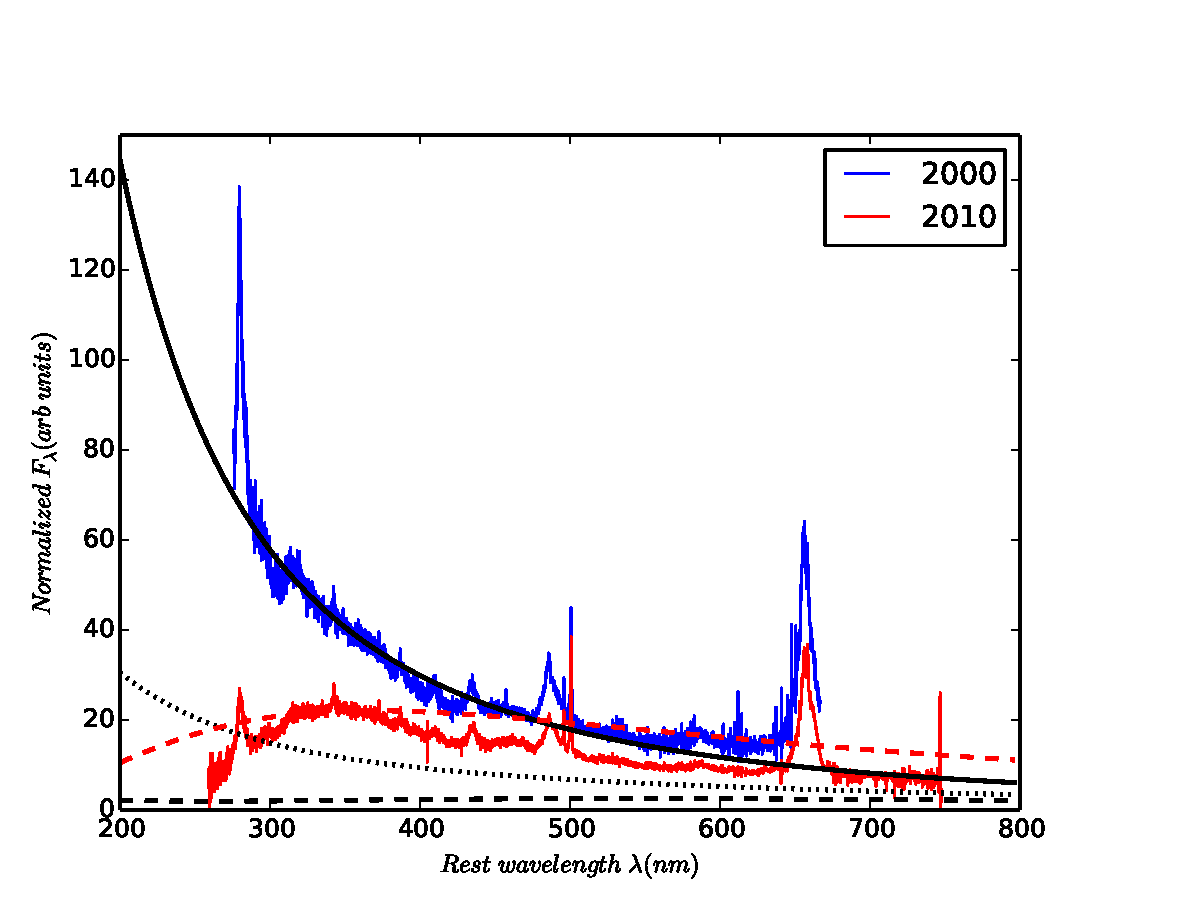
\includegraphics[width=8.7cm, trim=0.2cm 0.2cm 1.4cm 0.6cm, clip]
{../plots/models/mcd_gap_v3_3_b1.pdf}
\vspace{-12pt}
  \caption[]{
J1100-0053 data (blue line 2000 spectrum; red line 2010 spectrum) and
4 models. The solid black line shows non-zero torque at ISCO
\citep[following] []{Afshordi_Paczynski2003} while the
dashed black line shows a zero torque at the ISCO with a no absorption model. 
The green dashed line as a zero torque at the ISCO model multiplied by an 
absorption law adapted from \citep{Guo2016}.   }
  \label{fig:disk_suppression}
\end{figure}
Can J1100-0053 switch states from a thin disk quasar to an ADAF at
small radii with the thin disk surviving at large radii?
%%
Assuming the transition happens due to a thermal instability in the
inner disk on the thermal timescale, and propagates outwards to radii
$\sim$225$r_{g}$ as in \citet{Nemmen2006}, we can parameterize the
front propagation time as
\begin{equation}
    t_{\rm front}  \sim  5 \; {\rm yrs} \left(\frac{h/r}{0.1}\right)^{-1}
                                                           \left(\frac{\alpha}{0.3}\right)^{-1}  
                                                           \left(\frac{r}{225r_{g}}\right)^{3/2}  
                                                           \frac{r_{g}}{c}
\label{eqn:t_front}
\end{equation}
where we have had to assume a higher value of $\alpha \sim 0.3$
\citep{King2007} than typically assumed for thin ($h/r \ll 1$)
disks. This is plausible if there exists a very viscous disk and the
effect propagates outwards on a timescale of $\leq 5$ years from the
inner disk.

If the viscous disk switches to a RIAF at radii $<$225$r_{g}$, then
the UV/optical emission should be supressed by several orders of
magnitude compared to a radiatively efficient thin disk
\citep{Narayan1998, Abramowicz2002, Abramowicz2013}. However, if the
thin disk emission is simply uniformly suppressed within $<225r_{g}$
by a large factor, we cannot reproduce the shape of the 2010
J1100-0053 spectrum. Furthermore, in order to restore the thin disk in
the 2016 observation, a thermal instability is required to occur at
$\sim$225$r_{g}$ and a front to propagate inwards, collapsing the RIAF
back to a thin disk.

Noting RIAFs/ADAFs exist at lower luminosity than for a classic thin
disk ($\epsilon \sim 0.005$ and $\epsilon \sim 0.1$, respectively, for
$L=\epsilon \dot{M} c^{2}$) it is unclear first what physical
processes would trigger the change of state to an ADAF and then cool
back down to a thin disk, and second, why such an instability would
occur at the thin disk/RIAF boundary in J1100-0053, whereas in NGC
1097 this interface appears to be stable. In any case, suppressing the
MCD temperature profile inside a radius of $r_{{\rm alt}} = 225 r_{g}$
leads to a collapse in the total flux compared to unperturbed disk. 
%We show some example cases in Figure~\ref{fig:disk_suppression}. 
These scenarios are difficult to reconcile with our data.


\subsubsection{Propagation of a Cooling Front:}
Alternatively, a phenomenological explanation of the sequence of our
observations consists of a triggering event at the ISCO which cools
the inner disk and leads to the radial propagation outward of a
cooling front. At large radii, a heating front returns, re-inflating
the disk. This simple model, and our preferred model here, is outlined
in cartoon form in Figure~\ref{fig:J110057_diskmodel}.

Our explanation for the behaviour of J1100-0053 (and J2317+0005),
starts from the more-realistic, but $\alpha$-parameterized disk model
of \citet{Sirko_Goodman2003}. In their model, the outer accretion disk
is heated sufficiently to maintain stability against gravitational
collapse, and small changes in temperature can lead to large changes
in opacity and thus disk luminosity. In addition, the theoretical SEDs
have a second peak in the near-infrared that is energetically
comparable with the Big Blue Bump. \citet{Sirko_Goodman2003} assume
that the viscous torque at the inner edge of their accretion disks is
vanishingly small and effectively zero. This is a good assumption 
%for very thin disks and 
\emph{as long as there is no connection between
material inside the ISCO, i.e. the plunging region, and material at
the ISCO}.

An initially modestly fat disk ($h/r \sim 0.2$) with a modest
$\alpha$, cools from the ISCO and propagates outward in a cooling
front, collapsing the disk. The cooling (or indeed heating) front
propagates radially through an $\alpha$-parameterized disk at
approximately the sound speed $c_{\rm s}$ multiplied by $\alpha$
\citep[e.g., Eqn. 20 from][]{Hameury2009}  
\begin{equation}
v_{\rm front} = \alpha  c_{\rm s} 
\end{equation}
As the hot disk ($\sim 10^{5-6}$K) cools, it
fragments into cooler clumps around $\sim 10^{4}$K \citep[see e.g.,
][]{McCourt2016}.  
%%
Let us assume the cold phase clumps occur on size-scales of order
$r_g$, with an overdensity of $10^{4}$ relative to their surroundings,
and a relative velocity compared to the hot phase around them on the
order of the orbital velocity. Then, the cold phase clumps are
unstable to the Kelvin-Helmholtz instability
(Eqn.~\ref{eqn:T_cloudcrushing}) relative to their surroundings on an
approximate timescale of
\begin{equation}
t_{{\rm cc}} \approx 3{\rm mo} 
               \left( \frac{\rho_{\rm{cloud}}/\rho_{\rm{medium}}}{10^{4}}   \right)^{1/2}
               \left( \frac{r_{\rm cloud}}{r_{g}}\right) 
              \left( \frac{v_{\rm rel}}{10^{4}\rm{km s^{-1}}} \right)^{-1}.
\end{equation}
Our parameterization may not be particularly accurate but it is
illustrative. {\it The important point is that any cold phase clouds
must vanish after a relatively short time unless they are extremely
over-dense with very cold cores relative to the surrounding
medium.} 
}

The main coolants $>10^{4.5}$K are resonance lines
in Carbon and Oxygen and at lower temperatures, H and He from neutral
phase material \citep[see e.g., Fig. 18 in
][]{Sutherland_Dopita1993}. The ionization energies for carbon and
oxygen are 11.26 and 13.61 eV, respectively, i.e., $\sim 100$nm, and
hence at wavelengths $<100$nm the disk opacity will increase
dramatically in an edge.  However, the gas in the disk is pressure,
turbulence and Doppler broadened, so these ionization edges will
manifest around 100nm with decreasing opacity to shorter wavelengths
as
\begin{equation}
  \kappa \propto \rho T^{-1/2} \nu^{-3}
\end{equation}
for Kramers' opacities. This implies $\kappa \propto \lambda^{3}$
at increasing wavelengths up to the ionization edge around $100$nm.
These features will be blurred (by the broadening) and the ionization 
edges due to the C and O resonance lines in the cool phase of this
disk will be span $50-200$nm, depressing the flux at these energies. 
We note this closely resembles the opacity curve inferred by \citet{Guo2016} 
in J2317+0005 over relevant wavelengths.

The 2010 spectrum in this model comes from a cooler disk plus the
increased opacity at short wavelengths in the cooler phase. Heating
occurs from the outside in, explaining the 2016 spectrum and
asymmetric recovery in photometry.  Since the
optical continuum has been rising again since mid-2016, this leads to
a prediction of a rise in Hydrogen emission line flux in the next few
months. The infrared flux returns in 2021. 


However, if accretion disk luminosity is powered by magnetized gas
losing angular momentum, it is reasonable to assume that magnetic
fields are dragged across the ISCO with accreting matter, into the
plunging region. As a result, we should typically expect a non-zero
torque at the ISCO, as the magnetized plunging gas torques the ISCO
gas. A drop in the torque at the ISCO is then most likely due to a
change in $\dot{M}$ at the ISCO, which could result from a local
change in $\alpha$ or a stochastic variation in the mass supply. We
can regard this as the ``the triggering event''.



A non-zero torque at the ISCO implies that matter in the
plunging region is connected (however weakly) to matter outside the
ISCO, probably by magnetic fields \citet[e.g., ][]{Gammie1999,
Agol_Krolik2000}. A non-zero torque at the ISCO maintains a hotter
innermost disk than a condition of zero torque at the ISCO, and an
assumption of non-zero torque is particularly appropriate if disk
viscosity and accretion are driven by magnetic fields. Our model of
thermal emission from a MTB implies changes in the region from the
ISCO to $\sim$few tens-100 $r_{\rm g}$ are required to suppress flux
into the observed $g$-band. 

In particular, we suggest a physical
collapse of the disk scale height due to a cooling front propagating
outward from the ISCO. The radiation properties of accretion disk with
a NZTs at their inner edge was also explored by \citet{Cao2003} and
\citet{Cannizzo1998b} describe in detail, the change at the ISCO is
physically related to this thermal front.

\begin{figure*}
  %% trim=l b r t 
%  \includegraphics[width=15.4cm, height=18.75cm, trim=0.0cm 0.0cm 0.0cm 0.0cm, clip]
  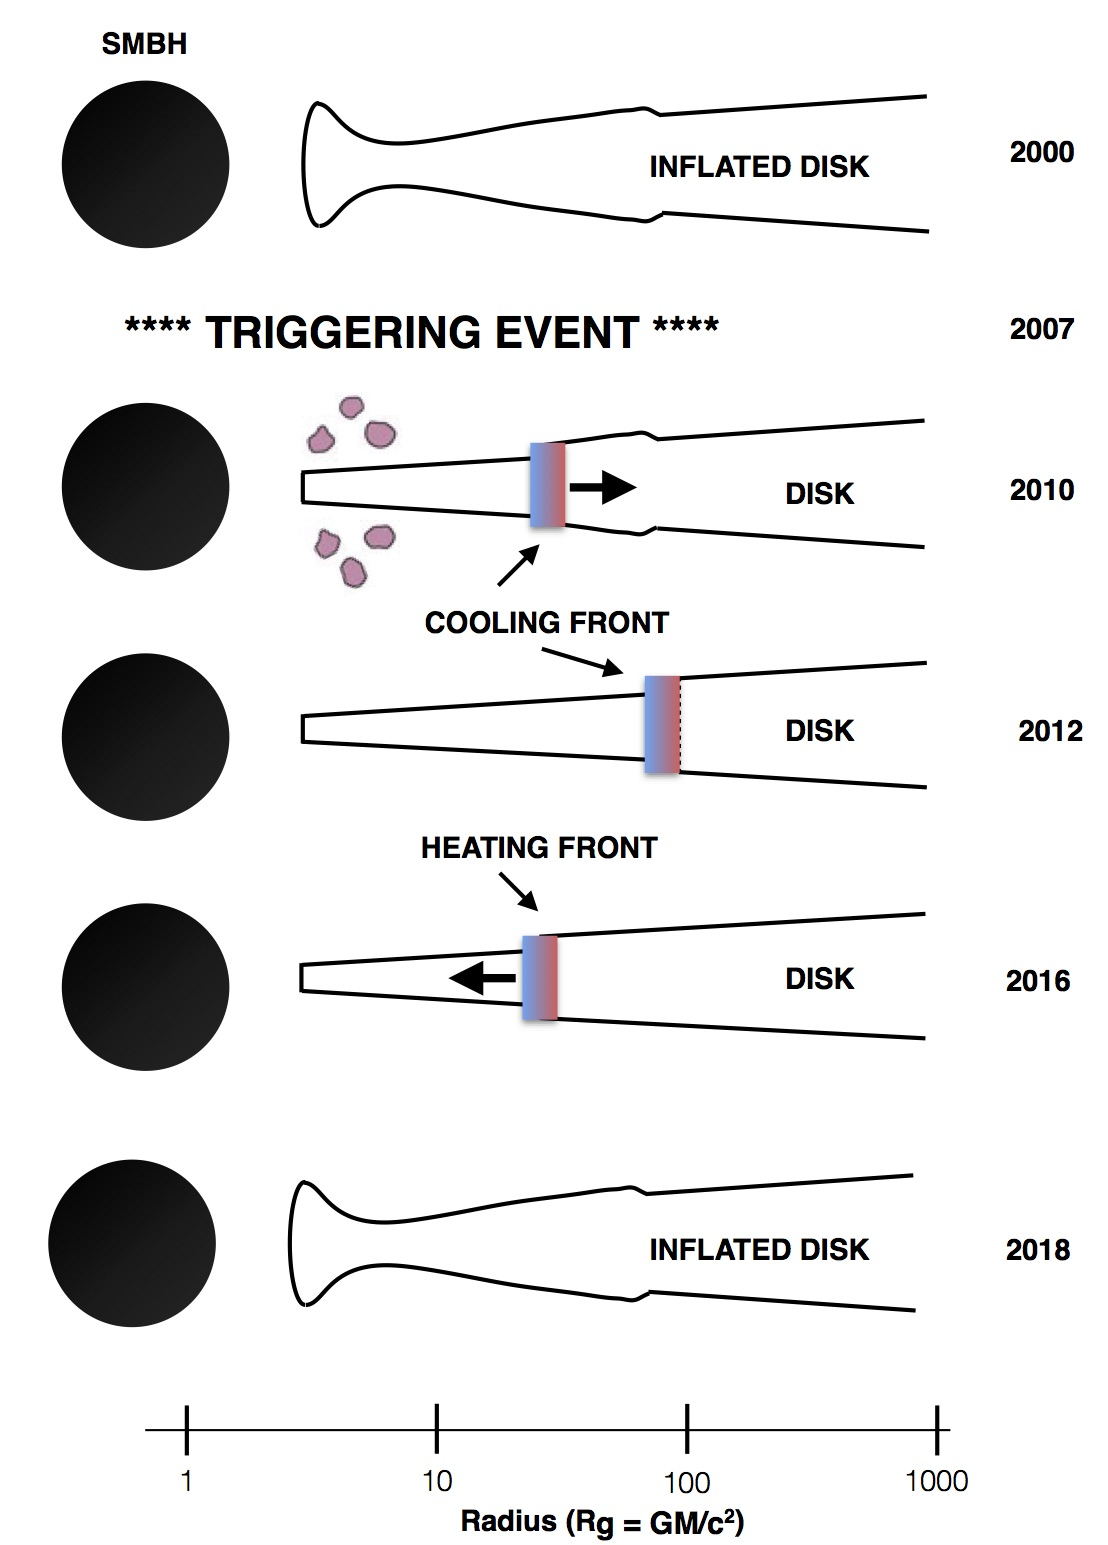
\includegraphics[width=15.4cm, trim=0.0cm 0.0cm 0.0cm 0.0cm, clip]
  {../plots/models/cartoon_v3pnt1.jpg}
  \centering
  \caption[]{
    Cartoon illustration of our model explaining the unusual spectral
evolution of J1100-0053. In 2000, corresponding to the SDSS spectral
epoch, the quasar has a standard inflated accretion disk, i.e., where
non-zero torque at the ISCO heats the inner radii of the accretion
disk, causing it to puff up \citep[e.g.,][]{Zimmerman2005}. Circa
2007, a triggering event occurs that deflates the inner disk, possibly
due to a shift in the magnetic field configuration leading to zero
torque at the ISCO.  This event leaves some scattering clouds, and
causing a cooling front to propagate outwards in the accretion disk,
traveling on the $t_{\rm front}$ time-scale 
\citep[see also][]{Hameury2009}. 
 Circa 2012, the cooling
front reaches a predicted kink in the accretion disk profile at
$\sim$100 $r_{g}$, associated with a shift in the accretion disk
opacity, e.g., Figure 2 of \cite{Sirko_Goodman2003}. A heating front
then travels radially inwards, re-heating the inner accretion disk but
on longer timescales, due to the thinner disk. We predict that in the
next year, the quasar should roughly return to its initial state.}
  \label{fig:J110057_diskmodel}
\end{figure*}

We note that \citet{Hameury2009} investigate thermal-viscous
instabilities in AGN, and find that a physical mechanism of
propogating cooling and heating fronts is found, and that these fronts
propagate on much shorter time scales than the viscous time.  The
model in \citet{Hameury2009} makes a firm prediction of this back and
forth propagation of cooling and heating fronts on a short time scale,
while noting that the surface density at smaller radii does not change
so quickly and hence $\dot{M}$ fluctuates on a longer timescale.

As noted above, one simple,
plausible trigger for this cooling front is that the non-zero torque
condition at theISCO changes to a (more nearly) zero-torque
condition. This dramatic decrease in the torque at the ISCO leads to a
drastically cooler, thinner innermost disk. As the cooling front
propagates, the drop in temperature leads to a drop in flux. To fit
the observed spectra, our model has the cooler regions behind the
front emitting 10\% the flux of the initial hotter disk, and assumes
the disk height drops by a factor $\sim$2. The dimming of the inner
disk causes a drop in the ionizing photon flux, which will cause the
Balmer lines to drop in flux after a light travel time of months and
the IR emission from the outer disk/torus to drop in flux after a
light travel time of $\sim$3 years \citep{Sirko_Goodman2003,
Koshida2014, Jun2015}.

If the inner accretion disk is usually inflated \citet[see e.g.,
][]{Sirko_Goodman2003, Thompson2005, Hopkins_Quataert2011}, such a
cooling front will naturally produce a collapse in the disk scale
height, triggering a decrease in flux moving from UV to longer optical
wavelengths, and a temporarily thicker scattering atmosphere, further
decreasing flux at short wavelengths (see
Fig.~\ref{fig:J110057_diskmodel}).  Given our disk parameters, outward
front propagation timescales are months-to-years, corresponding with
observed timescales for optical emission moving from shorter to longer
wavelengths as the radius of the cooling front increases. A decrease
in the UV flux would be expected to cause a decrease in IR flux, as
the heating of the IR-emitting dusty torus is reduced; however, there
should be a delay due to light travel time \citet[e.g.,
][]{Jun2015}. By 2010 (MJD 55300) the front has reached $r\sim50
r_{g}$. During that time, the collapsing disk height increases the
number density of scatterers and the temporary cold phase formed at
the disk surface produces the remarkable blue downturn in the 2010
spectrum. The cooling front continues to propagate radially outward
but cools less efficiently at larger disk radii.

Eventually, very much in the same vein as discussed by
\citet{Hameury2009}, somewhere in the disk, $\Sigma$ reaches the
critical surface density $\Sigma_{\rm max}$, and that triggers the
heating instability. A heating front propagates back inwards,
analagous to the well-known accretion disk limit cycle mechanism in
models of dwarf novae outbursts \citep[e.g.,][]{Cannizzo1998}. The
returning heating front travels more slowly because the disk is
thinner (and $t_{\rm front}$ is inversely proportional to $h/r$) and
will re-inflate the disk as it propagates inwards towards the
SMBH. This means the return to normal will be asymmetric in time, as
observed, and the shortest wavelength bands bottom out first, because
that wavelength is dominated by emission coming from $r\sim100r_{g}$.

Using \citet{Ford2018} and \citet{Sirko_Goodman2003},
Figure~\ref{fig:J110057_diskmodel} shows a model for a $M_{\rm
BH}=7\times 10^{8} M_{\odot}$, with an accretion rate in units of
Eddington accretion, $\dot{M}=0.070$ (appropriate for J1100-0053),
radiative efficiency of $\epsilon=0.1$ inner disk radius of $6r_{\rm
g}$ and outer disk radius of 10,000$r_{g}$. The resulting model
spectra can be seen in Figure~\ref{fig:J110057_spectra}. We expect the
front to return to the ISCO in mid-to-late 2018. That means the broad
Balmer lines will come back a few months later, but the WISE IR flux
should return to full flux in 2021. We note the IR brightness of
J2317+0005 was only observed at one epoch and the change in the UV for
J2317+0005 was rapid, decreasing by a factor of 3.5 at 3000\AA\ over
only 23 days. This indicates that the cooling event was very brief,
and given the extremal but plausible values of $h/r = 0.2-0.3$ and
$r=20-25$ with $\alpha$ held at 0.3, is consistent with our model.



%%%%%%%%%%%%%%%%%%%%%%%%%%%%%%%%%%%%%%%%%%%%%%%%%%%%%%%%%%%%%%%%%%%%%%%%%%%%%%%%%
%%%%%%%%%%%%%%%%%%%%%%%%%%%%%%%%%%%%%%%%%%%%%%%%%%%%%%%%%%%%%%%%%%%%%%%%%%%%%%%%%
%%
%%
%%   SECTION 4   SECTION 4   SECTION 4   SECTION 4   SECTION 4   SECTION 4  
%%   SECTION 4   SECTION 4   SECTION 4   SECTION 4   SECTION 4   SECTION 4  
%%   SECTION 4   SECTION 4   SECTION 4   SECTION 4   SECTION 4   SECTION 4  
%%
%%
%%%%%%%%%%%%%%%%%%%%%%%%%%%%%%%%%%%%%%%%%%%%%%%%%%%%%%%%%%%%%%%%%%%%%%%%%%%%%%%%%%
%%%%%%%%%%%%%%%%%%%%%%%%%%%%%%%%%%%%%%%%%%%%%%%%%%%%%%%%%%%%%%%%%%%%%%%%%%%%%%%%%%
\section{Conclusions} 
By monitoring changing look quasars we introduce new
tests of models of accretion disk physics. We present the 
quasar J1100-0053 that was catalogued in the Sloan Digital 
Sky Survey quasar survey, but identified as an interesting due 
to its near-infrared photometric properties. 

We have shown that a simple
phenomenological model with a propagating cooling front is capable of
describing the gross spectral and temporal variations in a changing
looking quasar. Our model makes a prediction for this source, testable
over the next few years and, if confirmed, implies that changing
looking quasars as a class are driven by changes near the ISCO, close
to the SMBH. The discovery of J1100-0053 (and J2317+0005) are specific
key examples of time-domain astronomy and the resulting astrophysics
to be studied. However, even with the coverage from WISE, PanSTARRS,
SDSS, DECaLS and CRTS, we have a relatively sparse dataset which
cannot tightly constrain our theoretical model. 

The Zwicky Transient
Facility \citep[ZTF; ][]{Bellm2014} has very recently started and will
open a new data space with high cadence, multi-band photometric
monitoring. Along with ZTF in the very near future, the Large Synoptic
Survey Telescope \citep{Ivezic2008, LSST_ScienceBookV2} will allow
identification of the types of events such as J1100-0053 and
J2317+0005 \emph{while they are occurring}, allowing spectroscopic
monitoring. We will be able to see how long a UV collapse lasts and
closely follow its evolution.  Such data will stringently test models
of AGN disks at much higher fidelity than we are able to do with
current `Changing-Look' quasar samples.

\smallskip
\smallskip
{\bf Author Contributions.}   
N.P.R. led the project, identified J1100-0053 as interesting, obtained and conglomerated the data, developed and wrote the manuscript and co-ordinated the team.
K.E.S.F. and B.K. orginated and developed the theoretical interpretation. 
M.G. and D.S. were heavily responsible for the initial discussions and observations that were the genesis of
this project, as well as being fully involved in preparing the manuscript. 
A.M.M. produced the initial infrared variable quasar catalogs, while DL provided the optical+infra image analysis. 
D.S., M.G. and A.J.D. were part of the Palomar observing team.
N.P.R., A.M.M. and A.D. are part of the DECaLS Legacy Survey. 
H.D.J. provided the Balmer line fits and contributed to the manuscript.
R.A. and A.D. significantly contributed to the manuscript.
\smallskip
\smallskip



\smallskip
\smallskip
{\bf Availability of Data and computer analysis codes}. 
All materials, data, code and analysis algorithms are fully 
available at: 
\href{https://github.com/d80b2t/WISE\_LCs}{\tt https://github.com/d80b2t/WISE\_LCs}


\smallskip
\smallskip



\section*{Acknowledgements}
NPR acknowledges support from the STFC and the Ernest Rutherford
Fellowship scheme.  KESF \& BM are supported by NSF PAARE
AST-1153335. KESF \& BM thank CalTech/JPL for support during
sabbatical.  MF acknowledges support from NSF grants AST-1518308,
AST-1749235, AST-1413600 and NASA grant 16-ADAP16-0232.  RJA was
supported by FONDECYT grant number 1151408. AMM acknowledges
support from NASA ADAP grant NNH17AE75I.

We thank David J. Schlegel for quality checks on the BOSS data, and
Chris Done for invigorating discussions at the concept and conclusion
of this work.

This publication makes use of data products from the Wide-field
Infrared Survey Explorer, which is a joint project of the University
of California, Los Angeles, and the Jet Propulsion
Laboratory/California Institute of Technology, and NEOWISE, which is a
project of the Jet Propulsion Laboratory/California Institute of
Technology. WISE and NEOWISE are funded by the National Aeronautics
and Space Administration.

This research has made use of the NASA/IPAC Extragalactic Database
(NED) which is operated by the Jet Propulsion Laboratory, California
Institute of Technology, under contract with the National Aeronautics
and Space Administration.

This research has made use of data obtained from the SuperCOSMOS
Science Archive, prepared and hosted by the Wide Field Astronomy Unit,
Institute for Astronomy, University of Edinburgh, which is funded by
the UK Science and Technology Facilities Council.

The GALEX GR6/7 Data Release hosted at
\href{http://galex.stsci.edu/GR6/}{http://galex.stsci.edu/GR6/} was
used. These data were obtained from the Mikulski Archive for Space
Telescopes (MAST). STScI is operated by the Association of
Universities for Research in Astronomy, Inc., under NASA contract
NAS5-26555. Support for MAST for non-HST data is provided by the NASA
Office of Space Science via grant NNX09AF08G and by other grants and
contracts.

Funding for SDSS-III has been provided by the Alfred P. Sloan
Foundation, the Participating Institutions, the National Science
Foundation, and the U.S. Department of Energy Office of Science. The
SDSS-III web site is
\href{http://www.sdss3.org/}{http://www.sdss3.org/}.
%%
SDSS-III is managed by the Astrophysical Research Consortium for the
Participating Institutions of the SDSS-III Collaboration including the
University of Arizona, the Brazilian Participation Group, Brookhaven
National Laboratory, Carnegie Mellon University, University of
Florida, the French Participation Group, the German Participation
Group, Harvard University, the Instituto de Astrofisica de Canarias,
the Michigan State/Notre Dame/JINA Participation Group, Johns Hopkins
University, Lawrence Berkeley National Laboratory, Max Planck
Institute for Astrophysics, Max Planck Institute for Extraterrestrial
Physics, New Mexico State University, New York University, Ohio State
University, Pennsylvania State University, University of Portsmouth,
Princeton University, the Spanish Participation Group, University of
Tokyo, University of Utah, Vanderbilt University, University of
Virginia, University of Washington, and Yale University.

\bibliographystyle{mnras}
\bibliography{/cos_pc19a_npr/LaTeX/tester_mnras}

% Don't change these lines
\bsp	% typesetting comment
\label{lastpage}
\end{document}

